\documentclass[aspectratio=169]{beamer}

% Choose how your presentation looks.
\mode<presentation>
{
    \usetheme{Darmstadt}      % or try Darmstadt, Madrid, Warsaw, ...
    \usecolortheme{wolverine} % or try albatross, beaver, crane, ...
    \usefonttheme{structurebold}  % or try serif, structurebold, ...
    \setbeamertemplate{navigation symbols}{}
    \setbeamertemplate{caption}[numbered]

%FrameNR
\setbeamertemplate{footline}{%
\begin{beamercolorbox}[wd=\paperwidth,ht=2.25ex,dp=1ex]{Grey}%
\hspace*{1ex} \insertframenumber{} / \inserttotalframenumber
\end{beamercolorbox}}%

    
    %Customerize Prasentation
    \definecolor{Grau}{HTML}{CCCCCC}
    \definecolor{GrauDark}{HTML}{777777} % auf weißem hintergrund
    \definecolor{Orange}{HTML}{EA5B10}
    \setbeamercolor{palette primary}{bg=Grau}
    \setbeamercolor{palette primary}{fg=Orange}
    \setbeamercolor{normal text}{fg=GrauDark}
    \setbeamercolor{structure}{fg=Orange} % farbe der items
    \setbeamertemplate{itemize item}[circle]
    \setbeamercolor{mini frame}{fg=Orange}
    \setbeamercolor{section in head/foot}{bg=Grau}
    \setbeamercolor{section in head/foot}{fg=Orange}
    \setbeamercolor{subsection in head/foot}{bg=white}
    \setbeamercolor{subsection in head/foot}{fg=GrauDark}
    \setbeamercolor{headline}{bg=Grau}
    \setbeamercolor{block body}{bg=white}
    \setbeamercolor{frametitle}{bg=white}
}

\usepackage[utf8]{inputenc}
\usepackage[T1]{fontenc}
\usepackage{ae}
\usepackage{ngerman}
\usepackage{calc}
\usepackage{graphicx}
\usepackage{makecell}
\usepackage{pgfplots}
\usepackage[autostyle=true,german=quotes]{csquotes}
\pgfplotsset{compat=1.4}

\newenvironment<>{varblock}[2][.9\textwidth]{%
    \setlength{\textwidth}{#1}
    \begin{actionenv}#3%
        \def\insertblocktitle{#2}%
        \par%
        \usebeamertemplate{block begin}}
    {\par%
        \usebeamertemplate{block end}%
\end{actionenv}}


\title{FreeJDAQ}
\subtitle{Visuelle Programmiersprache zur Datenerfassung auf
    einem Raspberry Pi}
\author{David Gawron, Stefan Geretschlaeger, Leon Huck,\\
 \underline{Jan Kublbeck}, \underline{Linus Ruhnke}}
\date{23. September 2019}

\begin{document}
    
    \begin{frame}
        \titlepage
    \end{frame}
    
    \section{Einleitung}
    
%Problemstellungsfolie
\begin{frame}{Einleitung}
	\frametitle{Problemstellung}
	\center
       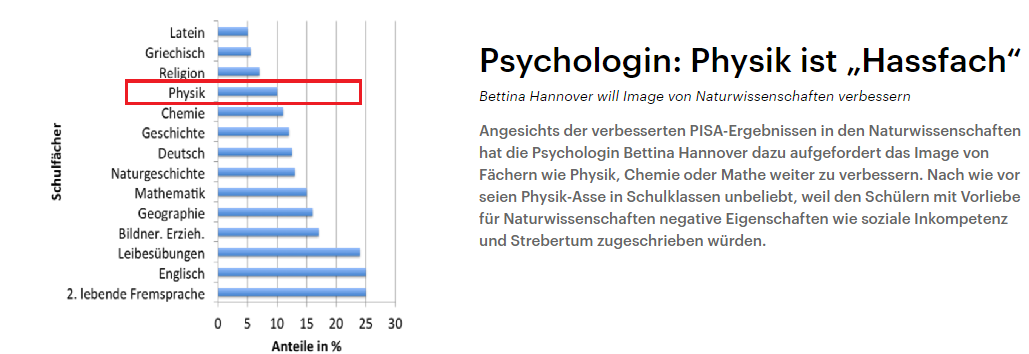
\includegraphics[width=\textwidth]{Grafiken/Physik7.png} \\
\end{frame}

\begin{frame}{Einleitung}
	\frametitle{Problemstellung}
	\center
       \includegraphics[width=7cm]{Grafiken/Physik4.png} \\
	\LARGE{Trotzdem: Lehrermangel in MINT-Fächern}
\end{frame}

\begin{frame}{Einleitung}
	\frametitle{Problemstellung}
	\center
       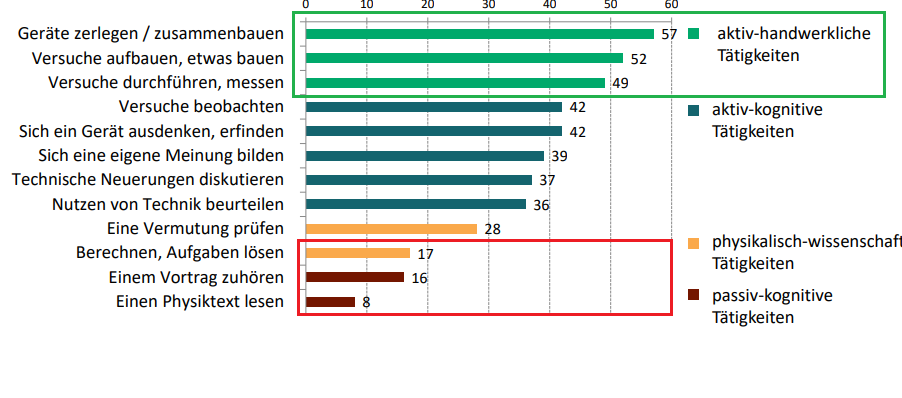
\includegraphics[width=\textwidth]{Grafiken/Physik1.png} \\
\end{frame}
    
 %Allgemeine Folie mit der Zielbestimmung als Einstieg
    \begin{frame}{Einleitung}
        \frametitle{Projektvorstellung}
        \center
        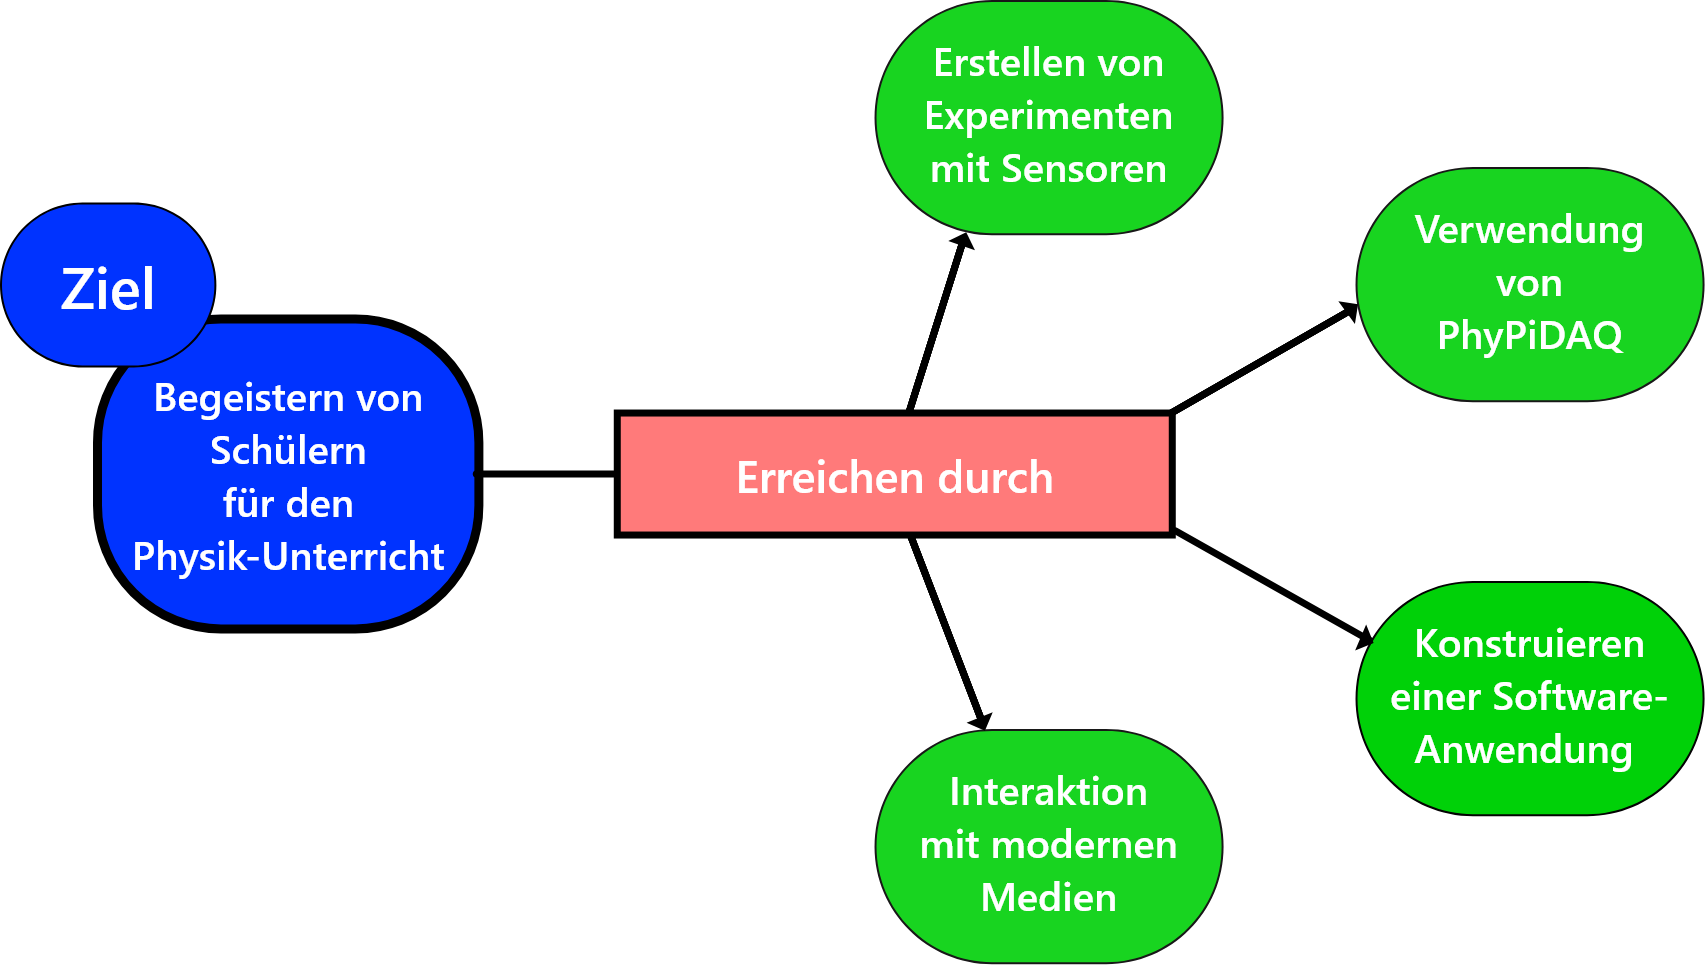
\includegraphics[width=\textwidth]{Grafiken/Ziel_Der_Anwendung.png} \\
    \end{frame}




%Erweiterungsmöglichkeiten von PhyPiDAQ
\begin{frame}{Einleitung}
    \frametitle{Erweiterungsmöglickeiten von PhyPiDAQ}
    \framesubtitle{Von Prof. Dr. Günter Quast}
    \center
    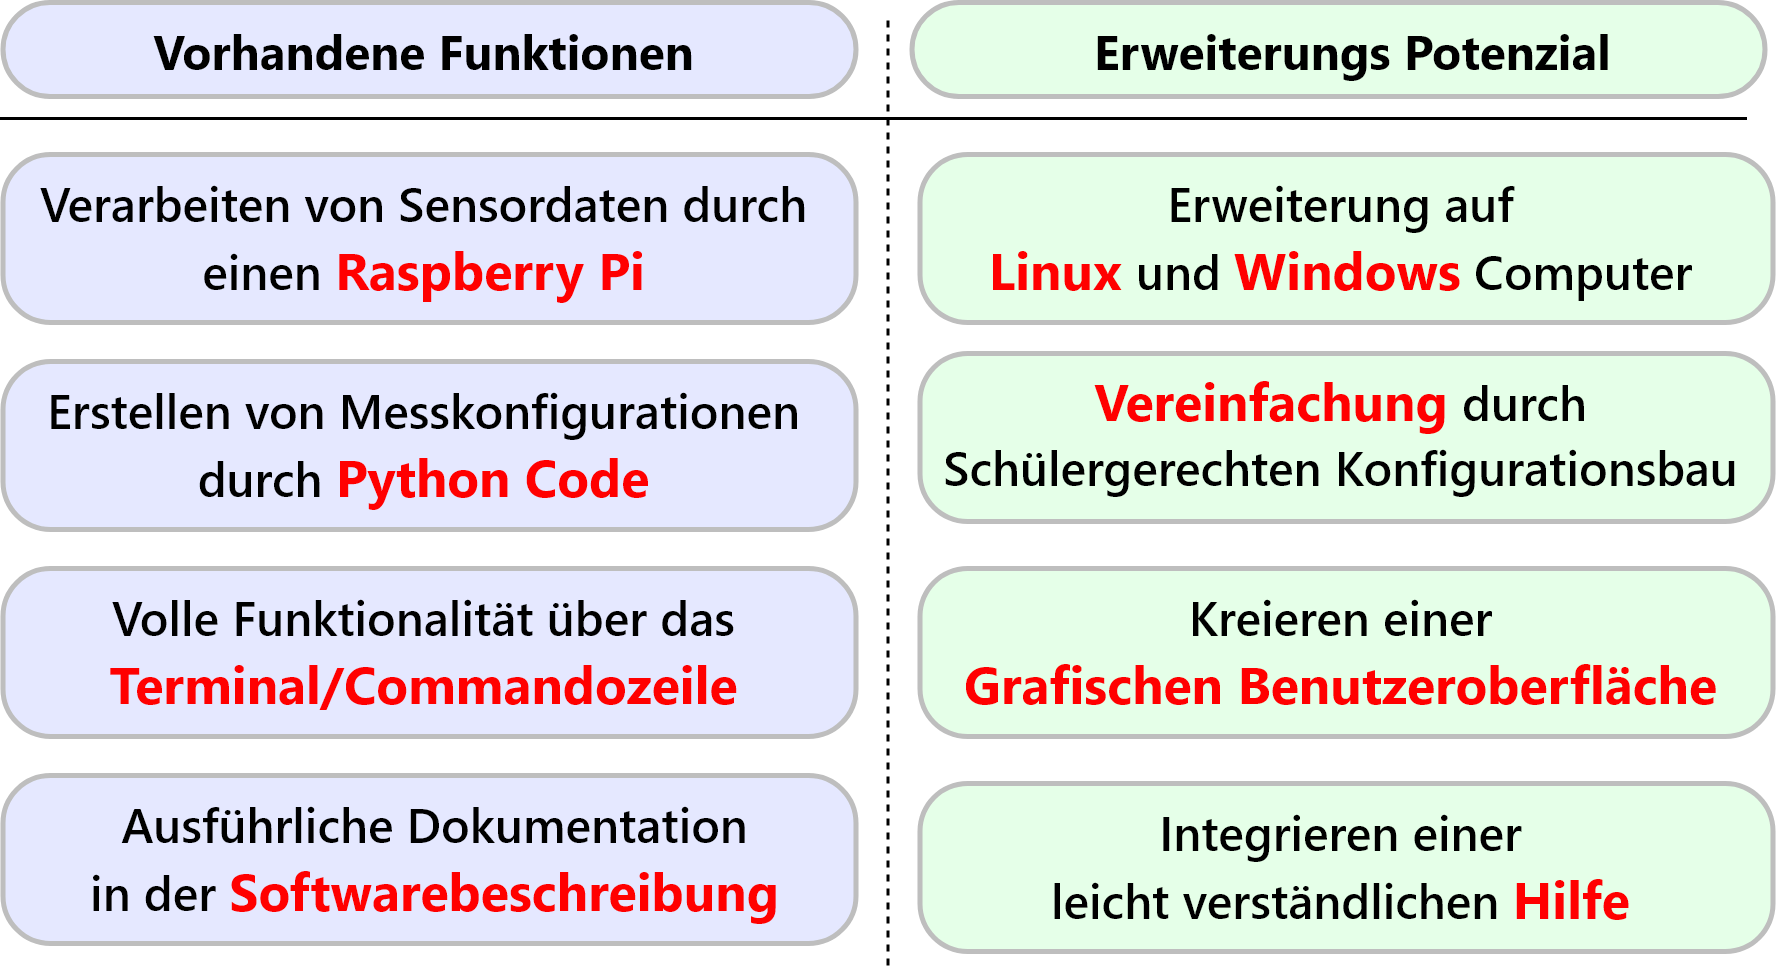
\includegraphics[width=\textwidth-2cm]{Grafiken/Gegenueberstellung_PhyPiDAQ_FreeJDAQ.png} \\
\end{frame}

    %FreeJDAQ Logo
    \begin{frame}{Einleitung}
        \frametitle{Projektvorstellung}
        \center
        
\includegraphics[width=5cm]{Grafiken/FreeJDAQ.png} \\
        \textbf{Free} \textbf{J}ava \textbf{D}ata \textbf{A}c\textbf{q}uisition
    \end{frame}


%GUI Erklärung
%\begin{frame}{Einleitung}
%    \frametitle{Funktionen des Konfigurations-Bereiches}
%    \center
%    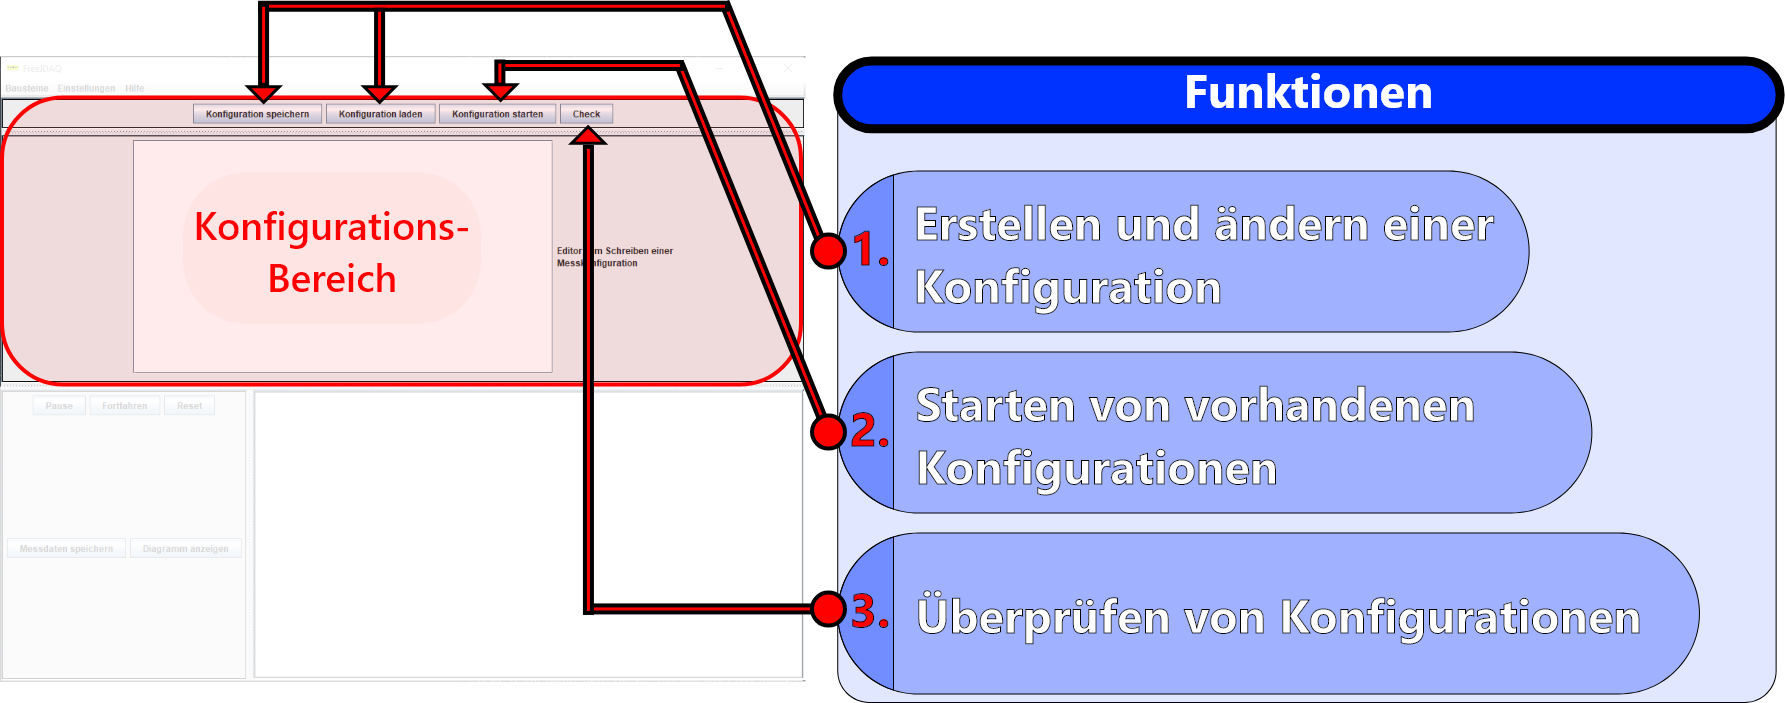
\includegraphics[width=\textwidth]{Grafiken/Funktionen_Des_Konfigurations-Bereiches.png} \\
%\end{frame}

%GUI Erklärung
%\begin{frame}{Einleitung}
%    \frametitle{Funktionen des Messlauf-Bereiches}
%    \center
%    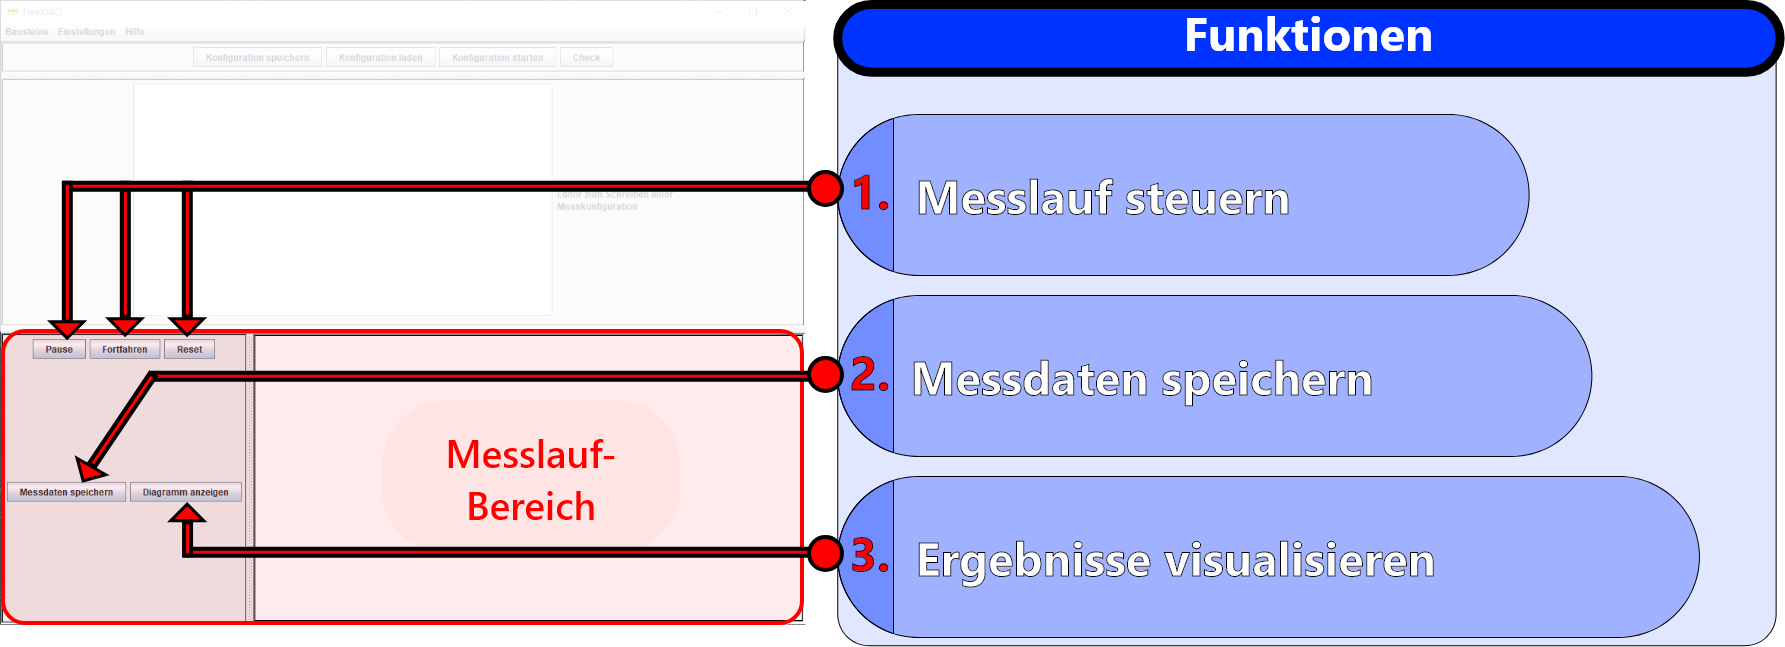
\includegraphics[width=\textwidth]{Grafiken/Messlauf-Bereich_Funktionen.png} \\
%\end{frame}

%GUI Erklärung
%\begin{frame}{Einleitung}
%    \frametitle{Funktionen des System-Bereiches}
%    \center
%    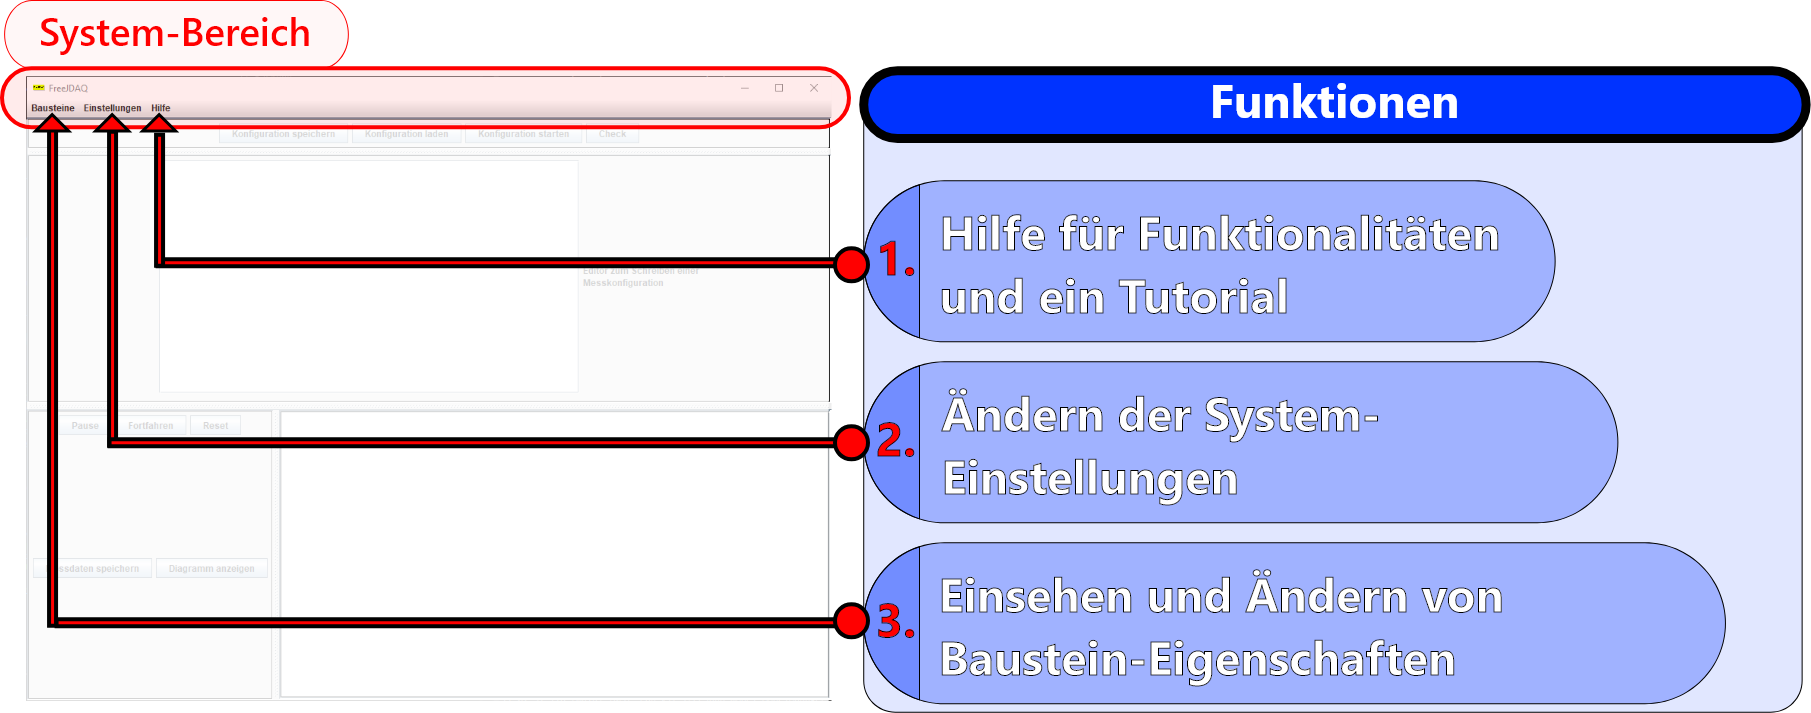
\includegraphics[width=\textwidth]{Grafiken/System-Bereich_Funktionen.png} \\
%\end{frame}

    \begin{frame}{Einleitung}
        \frametitle{Abgrenzungen}
        Was unser Produkt nicht enthält:
        \begin{itemize}
            \item Direkte Ansprache der Sensoren (PhyPiDAQ)
            \item Visuelle Repräsentation der Messkonfiguration
	     \item Abfangen von Fehlern beim Anschließen der Messtechnik
	     \item Erklärungen auf physikalischer Ebene
        \end{itemize}
    \end{frame}
    
    \section{Softwaretechnik}
    
    \begin{frame}{Softwaretechnik}
        \frametitle{Grundaufbau}
        \begin{center}
            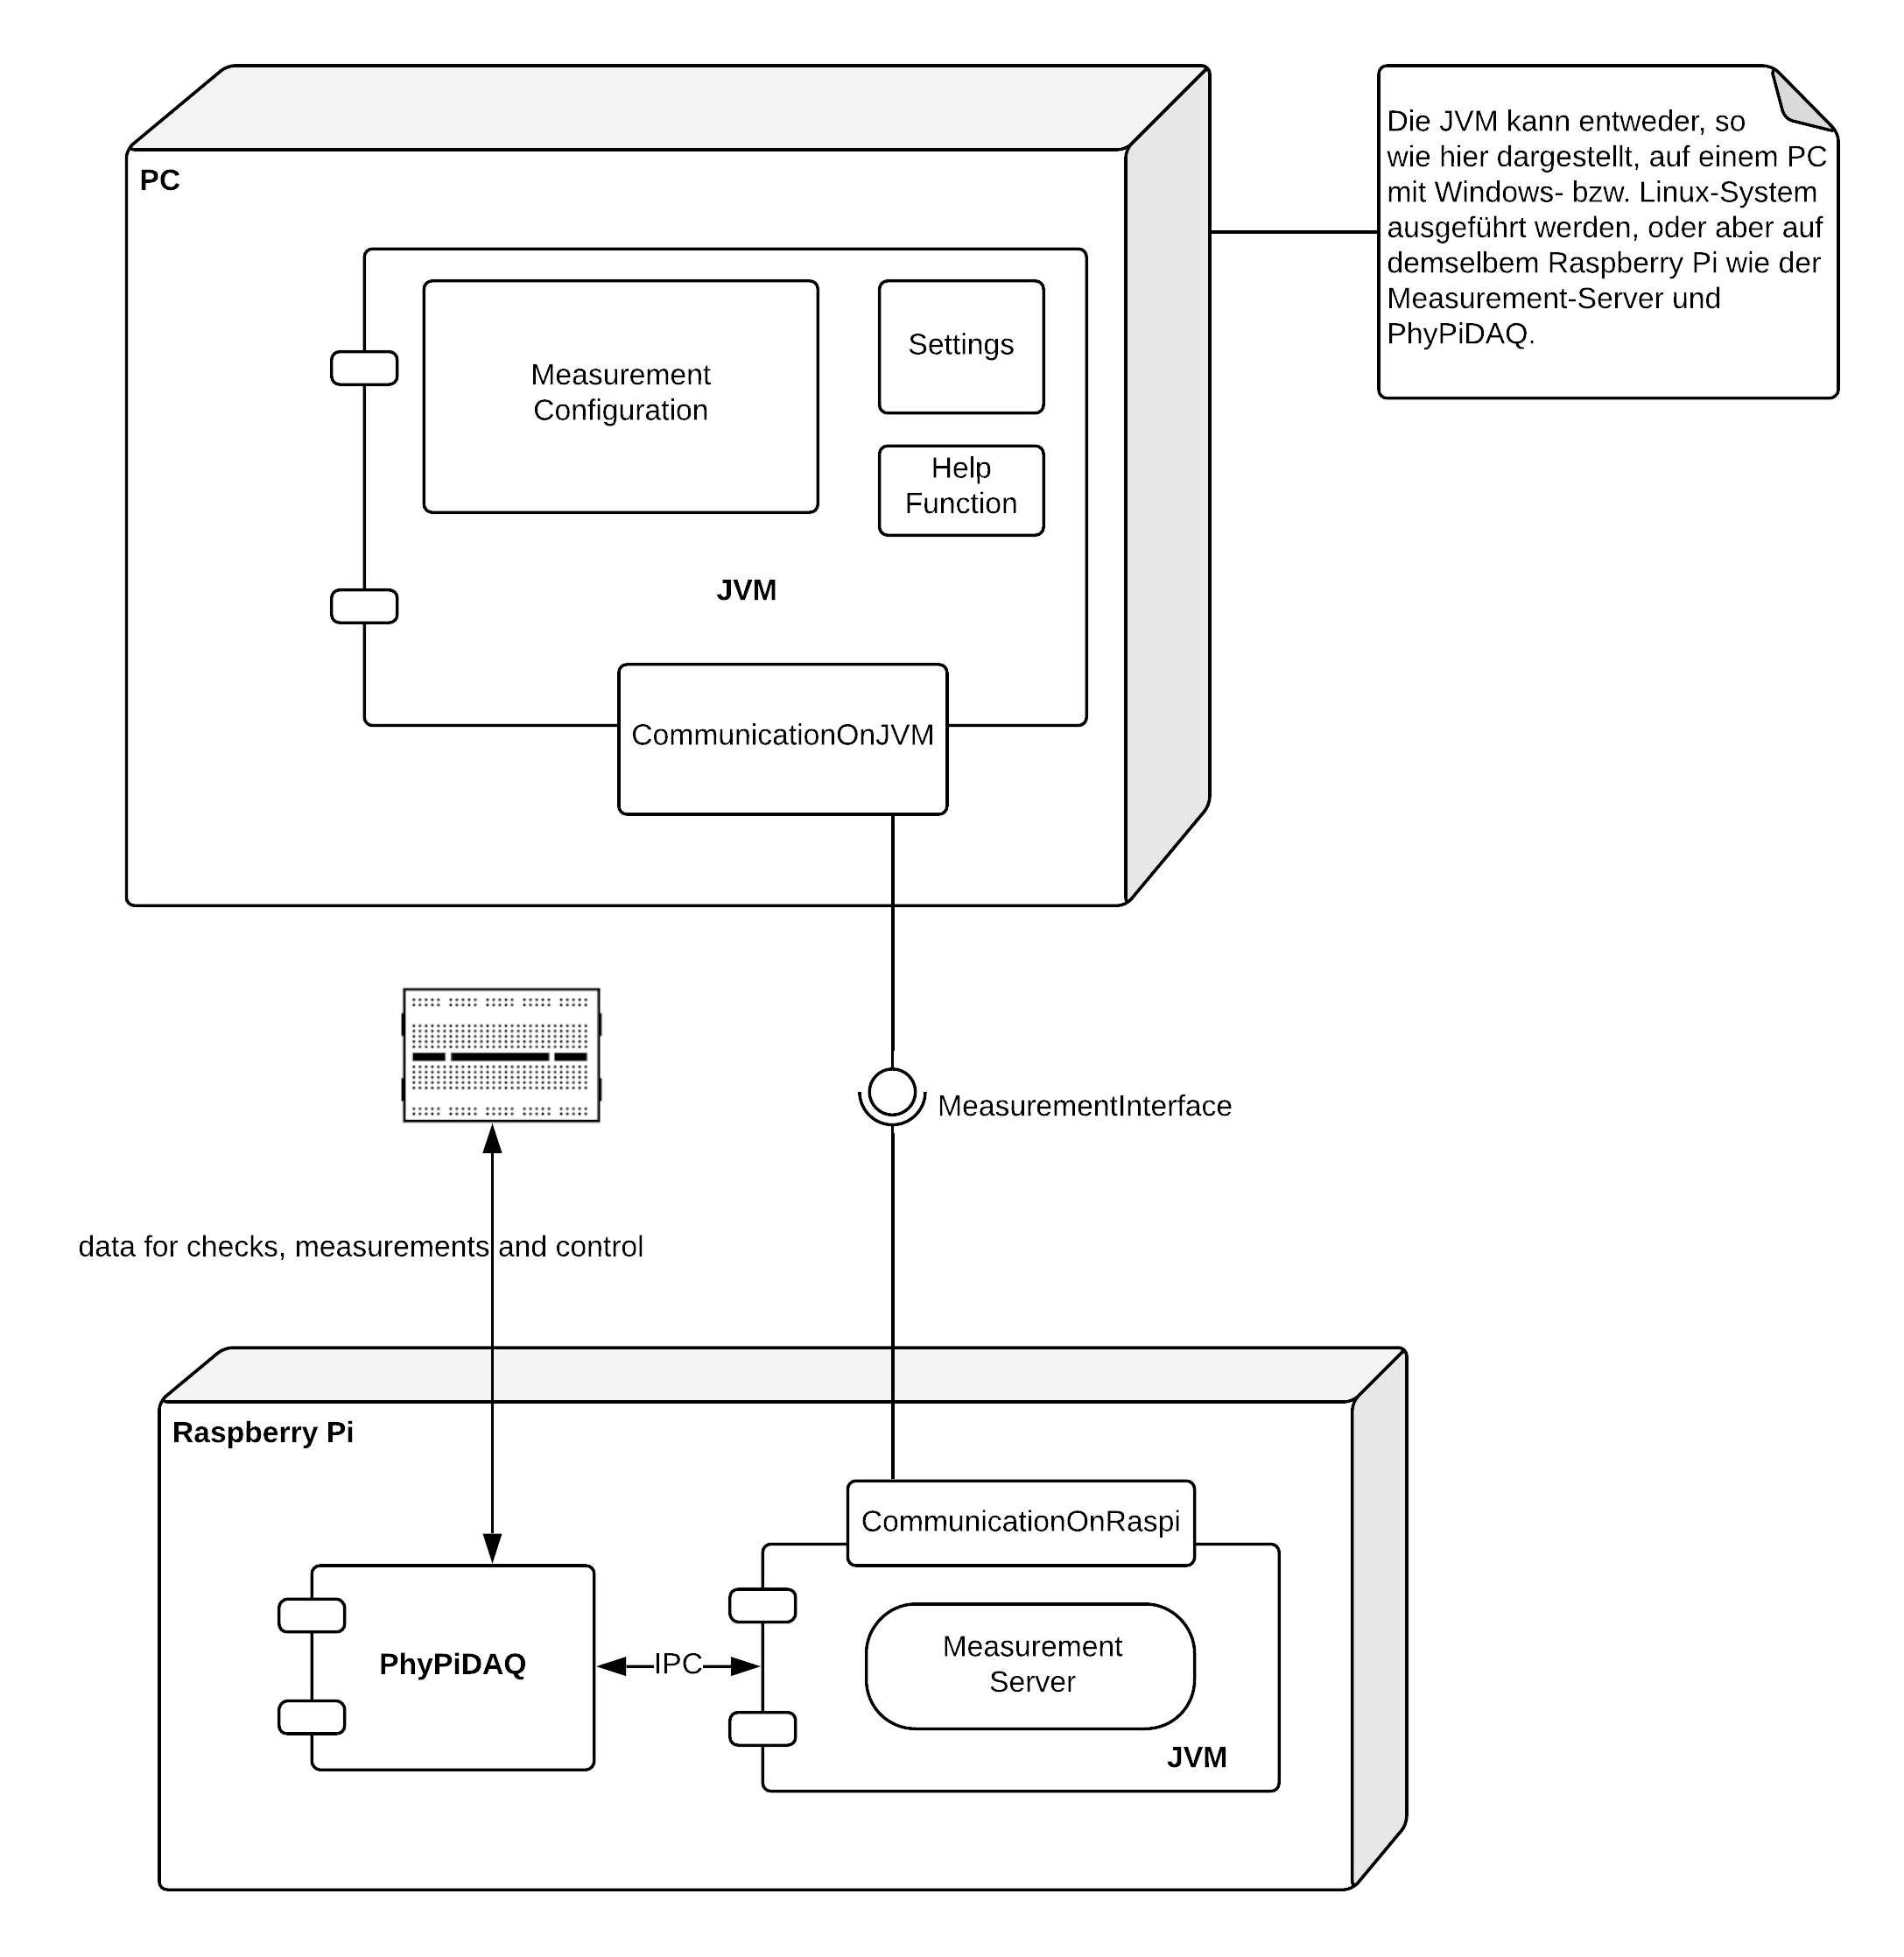
\includegraphics[width = 7cm,angle=90,origin=c]{Grafiken/DeploymentDiagram.png}
        \end{center}
    \end{frame}
    
    \begin{frame}{Softwaretechnik}
        \frametitle{Paketdiagramm}
        \begin{figure}[htbp]
            \begin{center}
                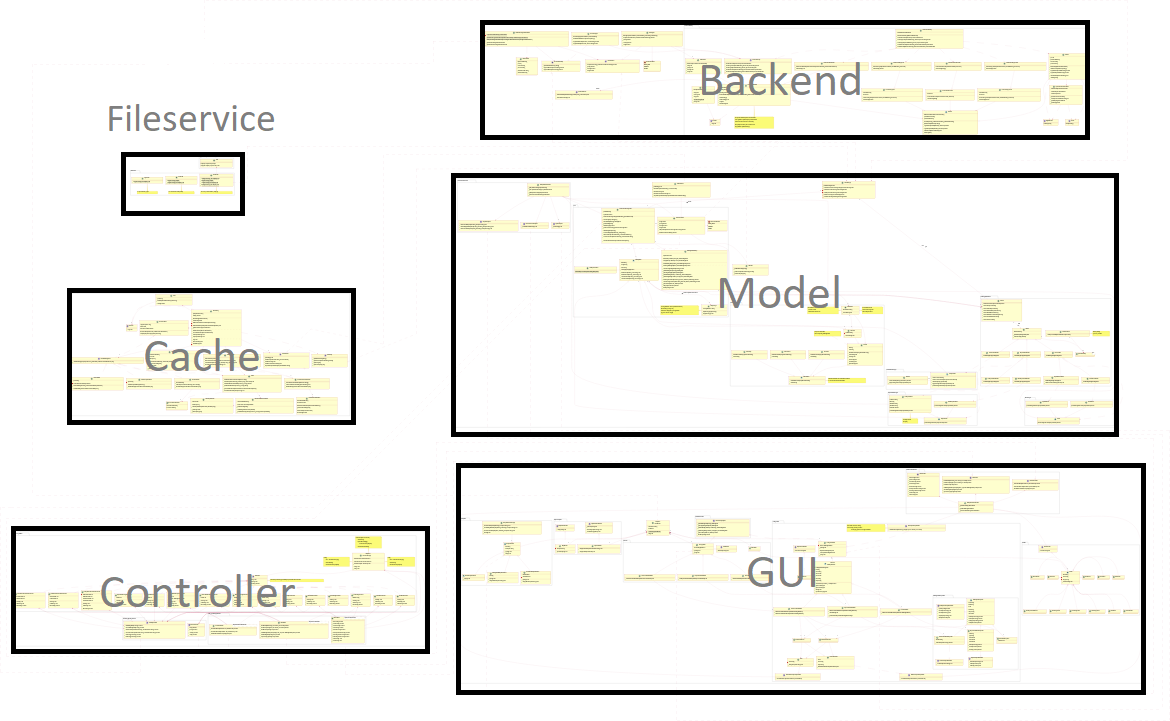
\includegraphics[width = 10cm]{Grafiken/Klassendiagramm.png}
            \end{center}
        \end{figure}
    \end{frame}
    
    \section{Statistiken}
    

    
    \begin{frame}{Statistiken}
        \frametitle{GitHub - FreeJDaq - Commits}
        \centering
        \begin{tikzpicture}
        \begin{axis}[
        ybar,
        enlarge x limits=0.2,
        width=0.95\textwidth,
        height=0.8\textheight,
        ylabel={Anzahl der Commits},
        xtick=data,
        nodes near coords,
        ymin=0,
        legend pos=north west,
        xticklabel style={rotate=45},
        symbolic x coords={1.7,8.7,15.7,22.7,29.7,5.8,12.8,19.8,26.8,1.9},xticklabels={1.7 (I),8.7,15.7,22.7,29.7,5.8 (Q),12.8,19.8,26.8,1.9 (IA)},
        ]
        
        \addplot coordinates
        {(1.7,6) (8.7,114) (15.7,123) (22.7,111) (29.7,205) (5.8,49) (12.8,72) (19.8,112) (26.8,29) (1.9,21)};
        \end{axis}
        \end{tikzpicture}
        Insgesamt 842 Commits, 54/64 Issues closed, (15.09, 18:00 Uhr)
    \end{frame}
    
    \begin{frame}{Lines of Code}
        \frametitle{GitHub - FreeJDaq - Lines of Code}
        \begin{table}[t]
            \begin{center}
                \begin{tabular}{ | l | c | }
                    \hline
                    Datei & Anzahl Zeilen \\
                    \hline
                    Anwendung & 4013 \\
                    Test & 1539 \\ \Xhline{0.8pt}
 			Java & 5552 \\ \Xhline{0.8pt}
                    Gesamt (inklusive Kommentar- und Leerzeilen) & 12776 \\ \hline
                \end{tabular}
            \end{center}
        \end{table}
	\center
        Verteilt über 122 Mainklassen und 23 Testklassen
    \end{frame}
    
    \begin{frame}{Unit-Tests}
        \centering
        \begin{tikzpicture}
        \begin{axis}[
        ybar,
        enlarge x limits=0.2,
        width=0.95\textwidth,
        height=0.8\textheight,
        ylabel={Anzahl},
        xtick=data,
        nodes near coords,
        ymin=0,
        legend pos=north west,
        xticklabel style={rotate=30},
        symbolic x coords={GUI,Controller,FileService,Cache,Model,Backend},xticklabels={GUI,Controller,FileService,Cache,Model,Backend},
        ]
        
        \addplot coordinates
        {(GUI,1) (Controller,7) (FileService,12) (Cache,3) (Model,66) (Backend,18)};
        \end{axis}
        \end{tikzpicture}
        Insgesamt 107 Testcases, zzgl. 33 GUI - Klickstrecken
    \end{frame}
    
    \begin{frame}{Statistiken}
        \frametitle{Testabdeckung}
        \centering
        \begin{tikzpicture}
        \begin{axis}[
        ybar,
        enlarge x limits=0.2,
        width=0.95\textwidth,
        height=0.8\textheight,
        ylabel={Prozent},
        xtick=data,
        nodes near coords,
        ymin=0,
        legend pos=north west,
        xticklabel style={rotate=30},
        symbolic x coords={Controller,FileService,GUI,Cache,Model,Backend},xticklabels={Controller,FileService,GUI,Cache,Model,Backend},
        ]
        
        \addplot coordinates
        {(Controller,53) (FileService,79) (GUI,84) (Cache,84) (Model,85) (Backend,96)};
        \end{axis}
        \end{tikzpicture}
        Insgesamt 80 Prozent Bedingungsüberdeckung.
       %Zweig-, Anwendungs-, einfache und mehrfache minimale Bedinungsüberdeckung
    \end{frame}
    
    \section{Tools}
    
    \begin{frame}{Tools}
        \frametitle{Allgemein}
        
        \begin{columns}
            \begin{column}{0.3\textwidth}
                \begin{block}{UML}
                    \center
                    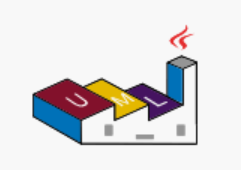
\includegraphics[width=(\textwidth / 2)]{Grafiken/PlantUmlIcon.png} %TODO find better logo
                \end{block}
            \end{column}
            \begin{column}{0.3\textwidth}
                \begin{block}{Unit-Testing}
                    \center
                    
\includegraphics[width=(\textwidth / 3)]{Grafiken/JUnitIcon.png}
                \end{block}
                \begin{block}{IDE}
                    \center
                    
\includegraphics[width=\textwidth / 4]{Grafiken/EclipseIcon.png}
                \end{block}
		\begin{block}{Java-Bibliotheken}
			\center
                    
\includegraphics[width=3cm]{Grafiken/SnakeYamlIcon.png}
                    
\includegraphics[width=3cm]{Grafiken/JFreeChartIcon.png}
                    
\includegraphics[width=(\textwidth / 4)]{Grafiken/SSHJIcon.png}
                \end{block}
                
            \end{column}
            \begin{column}{0.3\textwidth}
                \begin{block}{Build Management}
                    
\includegraphics[width=(\textwidth)]{Grafiken/MavenIcon.png}
                \end{block}
                \begin{block}{Statische Codeanalyse}
                    \center
                    
\includegraphics[width=(\textwidth / 4)]{Grafiken/JacocoIcon.png}
                    
\includegraphics[width=(\textwidth / 2)]{Grafiken/EclEmmaIcon.png}
                    
\includegraphics[width=(\textwidth / 2)]{Grafiken/SonarlintIcon.png}
                \end{block}
            \end{column}
        \end{columns}
    \end{frame}
    
    \section{Lernerfahrung}
    
    \begin{frame}
        \frametitle{Probleme}
        \begin{itemize}
            \item Teamkommunikation in den ersten Phasen 
            \item Nacharbeiten von Fehlern oder Vervollständigung
            \item Technologiewahl $\rightarrow$ Technologiewechsel
        \end{itemize}
    \end{frame}
    
    \begin{frame}
        \frametitle{Was haben wir gelernt}
        \begin{itemize}
            %Projektmanagement im allgemeinen
            \item Phasen planen  $\rightarrow$ Meilensteine, Deadlines setzen und Zuständigkeiten zuteilen
            \item Arbeitsverteilung gleichmäßig über den Zeitraum verteilen
            \item Meilensteine überprüfen und ggf. Ressourcen verschieben
            %Software-Entwicklung spezifisch
            \item Vor der Implementierung die nötigen Tools aussuchen und in diese einarbeiten
        \end{itemize}
	 \center
	 \includegraphics[width=8cm]{Grafiken/FreeJDAQCommits.png}
    \end{frame}
    
    \section{Livedemo}
    \begin{frame}[plain]
        \center
        {\huge Livedemo}
    \end{frame}

\appendix
\begin{frame}
        \frametitle{Zusammenfassung}
\textbf{Zur Anwendung:}
\begin{itemize}
	\item Es wurde eine Basis geschaffen, welche Schülern und Physikinteressierten Menschen eine Plattform gibt Messläufe einfach und schnell durchzuführen
	\item Weitere Produkteigenschaften und Erweiterungen können dieser Basis hinzugefügt werden
\end{itemize}
\textbf{Zur Gruppenarbeit:}
\begin{itemize}
	\item Trotz Schwierigkeiten während jeder Phase hat sich unsere Gruppendynamik dadurch positiv entwickelt
	\item Gewinnung wichtiger Erfahrung in der Projektplanung und Softwareentwicklung
        \end{itemize}
    \end{frame}

	
    \appendix
    \begin{frame}[plain]
	\center
	\huge{Vielen Dank für Ihre Aufmerksamkeit \\}

        
\includegraphics[width=5cm]{Grafiken/FreeJDAQ.png} \\
        \textbf{Free} \textbf{J}ava \textbf{D}ata \textbf{A}c\textbf{q}uisition
    \end{frame}
    
    \appendix
    \begin{frame}[plain]
        \frametitle{Quellen}
        \begin{itemize}
            \item https://github.com/osl2/DAQ-Documents
            \item https://github.com/osl2/PhyPiDAQ
            \item https://github.com/GuenterQuast/PhyPiDAQ
            \item http://plantuml.com/de/
            \item https://junit.org/junit5/
            \item https://www.eclipse.org/ide/
            \item https://bitbucket.org/asomov/snakeyaml/src
            \item https://github.com/hierynomus/sshj
            \item https://maven.apache.org/
            \item https://www.eclemma.org/
            \item https://www.eclemma.org/jacoco/
            \item https://www.sonarlint.org/
	     \item http://www.jfree.org/jfreechart/
        \end{itemize}
    \end{frame}

	\appendix
    \begin{frame}[plain]
        \frametitle{Quellen}
        \begin{itemize}
      \item {https://www.news4teachers.de/2019/08/lehrermangel-in-mint-faecher-ist-das-wissenschaftliche-niveau-in-der-lehrerausbildung-zu-hoch-debatte-um-reform-entbrannt/}
	\item https://bildungsluecken.net/307-wie-der-physik-lehrplan-den-spass-am-lernen-verdirbt

	% NEEDS FIX
	%\item https://www.kfp-physik.de/statistik/physikstudium_2017.pdf
	%\item https://ag4physik.files.wordpress.com/2017/03/interessensforschung_strahl.pdf
	%\item {http://www.physikdidaktik.info/data/_uploaded/Delta_Phi_B/2015/Caglar-Oeztuerk(2015)Interessenforschung_DeltaPhiB.pdf}
        \end{itemize}
    \end{frame}
    
\end{document}